% SmokeStream term project report. IEEE Computer Society journal template (IEEEtran, compsoc).
\documentclass[10pt,journal,compsoc]{IEEEtran}

\usepackage[T1]{fontenc}
\usepackage{graphicx}
\usepackage{booktabs}
\usepackage{amsmath}
\usepackage{array}
\usepackage{url}
\usepackage{tikz}
\usetikzlibrary{arrows.meta,positioning,fit,backgrounds}
\usepackage[hidelinks]{hyperref}

\graphicspath{{../figures/}}
\newcommand{\ugm}{\,\textmu g/m\textsuperscript{3}}

\begin{document}

\title{How Fast Can a Smoke Alert Be? The Latency--Accuracy Trade-off of Real-Time Wildfire Smoke Detection from Crowdsourced Sensor Streams}

\author{Vraj~Patel and Brandon~Moriguchi% <-- edit the author list if needed
\IEEEcompsocitemizethanks{\IEEEcompsocthanksitem Department of Applied Data Science, San Jos\'e State University, San Jos\'e, CA, USA. DATA 226 term project, Fall 2026.\protect\\
Code: \url{https://github.com/VRAJ8/smokestream}}}

\IEEEtitleabstractindextext{%
\begin{abstract}
Low-cost PurpleAir sensors are how many people in the western United States check wildfire smoke, yet the methods that turn their readings into trusted numbers were validated in hindsight, on complete data. A real-time system must decide while readings arrive late, sensors drop out and fire and plume data are hours old. We measure what deciding in real time costs. We built a streaming pipeline (Kafka, Spark Structured Streaming, MongoDB Atlas, Snowflake, Airflow) that corrects and quality-checks sensor readings and uses fire, smoke-plume and wind context to separate wildfire smoke from local pollution, and a batch pipeline that runs identical code with full hindsight. A simulator of Spark's watermark semantics, validated to reproduce the engine's output exactly, makes season-scale sweeps possible. Replaying the 2020 Bay Area fire season and three short event windows with arrival delays measured from the live sensor network, we find that late data costs almost nothing (at most 0.61\ugm{} from hindsight, against a 17.4\ugm{} sensor-to-monitor error), while stale context costs most: refreshing fire and plume data every 6 hours instead of every 15 minutes cuts label agreement from 92\% to 84\%, and to 55\% on July 4, 2021. Smoke alerts were 88\% precise in 2020 and arrived a median 99 minutes before the official hourly value. We add bounded-memory stream summaries (Bloom filter, Flajolet--Martin, DGIM, reservoir sampling), LSH over sensor-day curves, a k-anonymity and differential-privacy analysis of publishing hexagon data, and a data-poisoning test that shows where the neighbour check fails.
\end{abstract}

\begin{IEEEkeywords}
Stream processing, watermarks, Apache Spark, Apache Kafka, wildfire smoke, low-cost sensors, streaming algorithms, locality-sensitive hashing, differential privacy, data poisoning.
\end{IEEEkeywords}}

\maketitle
\IEEEdisplaynontitleabstractindextext
\IEEEpeerreviewmaketitle

\section{Introduction}
\IEEEPARstart{O}{n} September 9, 2020, the sky over the San Francisco Bay Area turned orange. Lightning had started dozens of fires around the region, and a regulatory monitor in Santa Cruz County beside the CZU Lightning Complex recorded hourly PM\textsubscript{2.5} of 826\ugm, about fifteen times the threshold for ``Unhealthy'' air. For many residents the most immediate information came not from the handful of regulatory monitors but from thousands of crowdsourced PurpleAir sensors and the maps that correct and display them.

Those maps are real-time systems, and every real-time system makes choices its users never see: how long to average readings, how long to wait for late data, how much history a sensor needs before it is trusted, and how stale fire and plume data may be. For a data engineer these are the familiar controls of stream processing, namely windows, watermarks and state~\cite{akidau2015dataflow}. For the public they decide whether an alert arrives early enough to act on, or is a false alarm that teaches people to ignore the next one. The correction and quality-control methods behind the maps were validated on complete data~\cite{barkjohn2021,barkjohn2022}; to our knowledge nobody has measured what processing in real time costs.

We ask four research questions. \textbf{RQ1:} how much accuracy and alert reliability does streaming lose against full hindsight on the same data? \textbf{RQ2:} how do window size, late-data tolerance (watermark), quality-check history and context freshness trade latency against accuracy? \textbf{RQ3:} can in-stream context separate wildfire smoke from local spikes such as fireworks? \textbf{RQ4:} can the pipeline sustain accelerated replay within a latency target on one laptop?

Our contributions are: (1) a measurement methodology (delay-aware replay with arrival delays measured from the live network, shared streaming and batch code, and held-out evaluation against regulatory monitors); (2) a simulator of Spark's watermark semantics that reproduces the engine window for window in seconds instead of hours, and two pitfalls it exposed; (3) the latency--accuracy frontier across four knobs on the 2020 season and three event windows; and (4) four course techniques applied where the problem needs them: stream summaries for duplicate delivery, sensor counts, alert persistence and labeling samples; LSH to find sensors that move together; k-anonymity and differential privacy for publishing data from sensors at people's homes; and a data-poisoning test of the quality check.

\section{Related Work}\label{sec:related}
\subsection{Wildfire smoke and its measurement}
Smoke exposure harms respiratory health~\cite{reid2016}, has risen sharply across the United States~\cite{burke2021}, and has reversed much of the improvement in PM\textsubscript{2.5} in western states~\cite{burke2023}. Machine-learning models estimate daily smoke PM\textsubscript{2.5} on a 10\,km grid~\cite{childs2022} and fuse low-cost sensors into exposure models~\cite{bi2020}, but they are retrospective and daily. Satellite products supply the context we use: VIIRS 375\,m active-fire detections~\cite{schroeder2014} and analyst-drawn NOAA Hazard Mapping System smoke plumes~\cite{rolph2009}. The public AirNow Fire and Smoke Map~\cite{firemap} shows corrected sensors next to these layers, but its processing settings are fixed and their accuracy cost is not reported.

\subsection{Correcting low-cost sensors}
PurpleAir sensors overestimate PM\textsubscript{2.5}, especially in smoke~\cite{holder2020,delp2020}. Barkjohn et al.\ developed the U.S.-wide correction used on the Fire and Smoke Map~\cite{barkjohn2021} and extended it to extreme smoke~\cite{barkjohn2022}. Crowdsourced data has also shown how smoke penetrates indoors~\cite{liang2021}. All of this work evaluates corrections on complete, after-the-fact data; we re-validate the correction on our sample (Section~\ref{sec:data}) and then ask what real time costs on top of it.

\subsection{Stream processing and event time}
Kafka~\cite{kreps2011} and Spark Structured Streaming~\cite{armbrust2018}, which grew out of discretized streams~\cite{zaharia2013}, are the standard open tools for fault-tolerant streaming; Flink~\cite{carbone2015} and MillWheel~\cite{akidau2013} offer similar event-time models. The Dataflow model frames stream processing as a balance of correctness, latency and cost, with windows, watermarks and triggers as the controls~\cite{akidau2015dataflow}. Lambda and Kappa architectures describe how batch and streaming views coexist~\cite{marz2015,kreps2014}; our hindsight baseline is the batch view of a Lambda design, used as a yardstick. Streaming benchmarks measure throughput and latency of engines on synthetic workloads~\cite{chintapalli2016,karimov2018}; we instead measure the accuracy cost of the engine's semantics on a real workload.

\subsection{Streaming algorithms and similarity search}
Bounded-memory summaries answer queries over unbounded streams~\cite{leskovec2020}: Bloom filters for membership~\cite{bloom1970}, Flajolet--Martin sketches for distinct counts~\cite{flajolet1985}, the DGIM algorithm for counts over sliding windows~\cite{datar2002}, and reservoir sampling for uniform samples of unknown-length streams~\cite{vitter1985}. Locality-sensitive hashing finds similar items without comparing every pair~\cite{indyk1998}; random-hyperplane hashing (SimHash) approximates cosine similarity~\cite{charikar2002}.

\subsection{Privacy and data integrity in crowdsourced sensing}
k-anonymity~\cite{sweeney2002} and l-diversity~\cite{machanavajjhala2007} limit re-identification through generalization; differential privacy bounds what any one contributor changes in a release by adding calibrated noise~\cite{dwork2006,dwork2014}. Open sensor networks also invite false data: poisoning attacks corrupt learned models~\cite{biggio2012}, and one party controlling many identities defeats majority-based checks (the Sybil attack~\cite{douceur2002}). We test both ideas against a quality check designed for faulty, not malicious, sensors.

\section{Data}\label{sec:data}
The study area is the Bay Area (36.9--38.3\textdegree N, 123.0--121.2\textdegree W). Table~\ref{tab:seasons} summarizes the ground truth and context for three fire seasons, and Fig.~\ref{fig:season} shows the 2020 season.

\begin{table}[t]
\caption{Fire seasons in the study area. Unhealthy: hourly PM\textsubscript{2.5} above 55.4\ugm{} at a regulatory monitor. Plume day: HMS smoke over at least half of the region. Fires within about 150\,km.}
\label{tab:seasons}
\centering\footnotesize
\setlength{\tabcolsep}{3pt}
\begin{tabular}{lrrrrrr}
\toprule
Season & Sites & Unhealthy h & Episodes & Peak \ugm & Plume days & Fires \\
\midrule
2020 & 20 & 3,327 & 371 & 826 & 48 & 85,660 \\
2021 & 19 & 155 & 51 & 182 & 58 & 25,014 \\
2024 & 19 & 12 & 6 & 222 & 46 & 2,721 \\
\bottomrule
\end{tabular}
\end{table}

\begin{figure}[t]
\centering
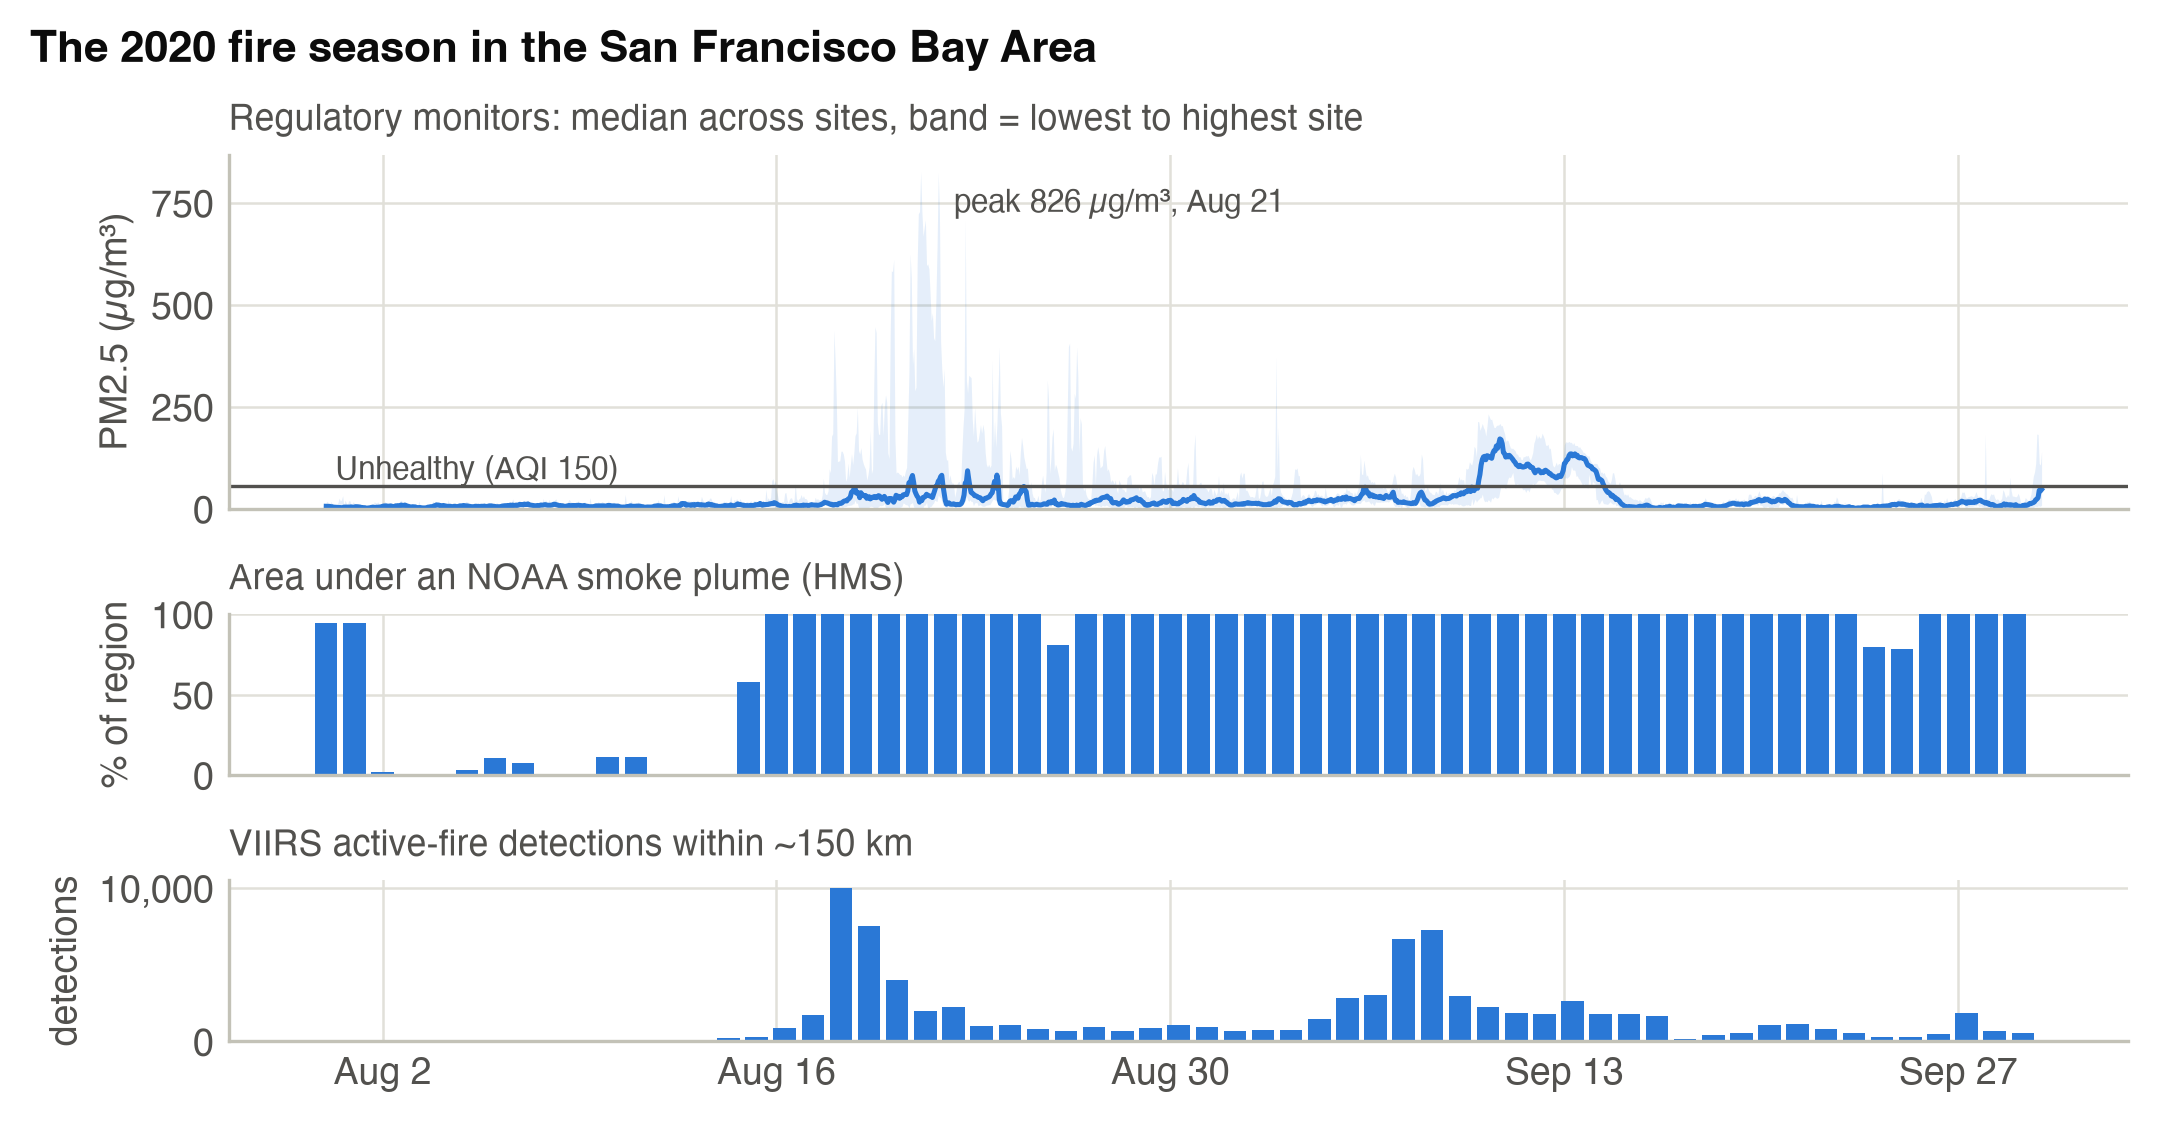
\includegraphics[width=\columnwidth]{season_2020}
\caption{The 2020 season: monitor PM\textsubscript{2.5} (median and range across 20 sites), share of the region under an HMS plume, and daily VIIRS fire detections.}
\label{fig:season}
\end{figure}

\textbf{Ground truth and context} are public and free: EPA AQS hourly PM\textsubscript{2.5} at regulatory monitors (held out, never read by the pipelines), NASA FIRMS VIIRS fire detections, NOAA HMS smoke polygons converted to H3 cells~\cite{h3}, and ASOS airport wind. Plume overlap alone cannot tell smoke at ground level from smoke aloft: plumes covered more than half the region on 46 days in 2024, a season with almost no wildfire smoke at the surface.

\textbf{Sensor history} costs points per row from the PurpleAir API, so we spend it where it matters: 10-minute data for the 2020 peak (August 16 to September 15; 40 sensors, 143,748 readings) and three four-day event windows: July 3--6, 2021 and 2024 (fireworks, the local-pollution test for RQ3; 26 and 28 sensors) and August 26--29, 2021 (Caldor fire smoke; 29 sensors). Sensors are sampled around each monitor (up to two within 5\,km), because a random sample left 15 of 20 monitors with no sensor nearby.

\begin{table}[t]
\caption{PurpleAir history used (10-minute averages). QC pass: readings that pass the range and channel-agreement checks. Points: API cost, measured at 4 points per row plus 2 per request.}
\label{tab:purpleair}
\centering\scriptsize
\setlength{\tabcolsep}{3pt}
\begin{tabular}{llrrrr}
\toprule
Run & Dates & Sensors & Readings & QC pass & Points \\
\midrule
2020 peak & Aug 16--Sep 15, 2020 & 40 & 143,748 & 86.2\% & 576k \\
July 4, 2021 & Jul 3--6, 2021 & 26 & 14,365 & 94.8\% & 58k \\
Caldor smoke & Aug 26--29, 2021 & 29 & 16,477 & 89.1\% & 66k \\
July 4, 2024 & Jul 3--6, 2024 & 28 & 15,535 & 90.1\% & 62k \\
\bottomrule
\end{tabular}
\end{table}

\textbf{Correction.} Against 7,890 monitor-hours at 16 monitors, the EPA U.S.-wide linear correction~\cite{barkjohn2021} matched the monitors (bias $-0.6$\ugm, $R^2=0.83$), while a piecewise ``extended'' form found in public tools overestimated smoke-level concentrations by 46--67\% and uncorrected sensors read 1.7--2.1 times high. We use the linear form.

\textbf{Arrival delays} were measured by polling 200 live sensors every 5 minutes (207 usable poll pairs, 43,600 samples, October 2026): readings were a median 79.5\,s old when polled (95th percentile 141\,s), and 98 sensor outages were observed. The replay draws from this profile: a reading with event time $e$ arrives at
\begin{equation}
a = e + \delta, \qquad \delta \sim \hat F_{\text{staleness}},
\end{equation}
where $\hat F_{\text{staleness}}$ is the empirical distribution of the 101 measured quantiles, and each sensor starts an outage at the observed rate ($7.9\times10^{-6}$ per sensor-second) for a duration drawn from the observed outages.

\section{System}
Fig.~\ref{fig:flow} shows the flow. The replay tool re-sends historical readings in arrival order: each reading's arrival time is its event time plus a delay drawn from the measured profile, with outages injected at the observed rate. It writes to Kafka at a chosen speed, or to one file per simulated minute.

\begin{figure*}[t]
\centering
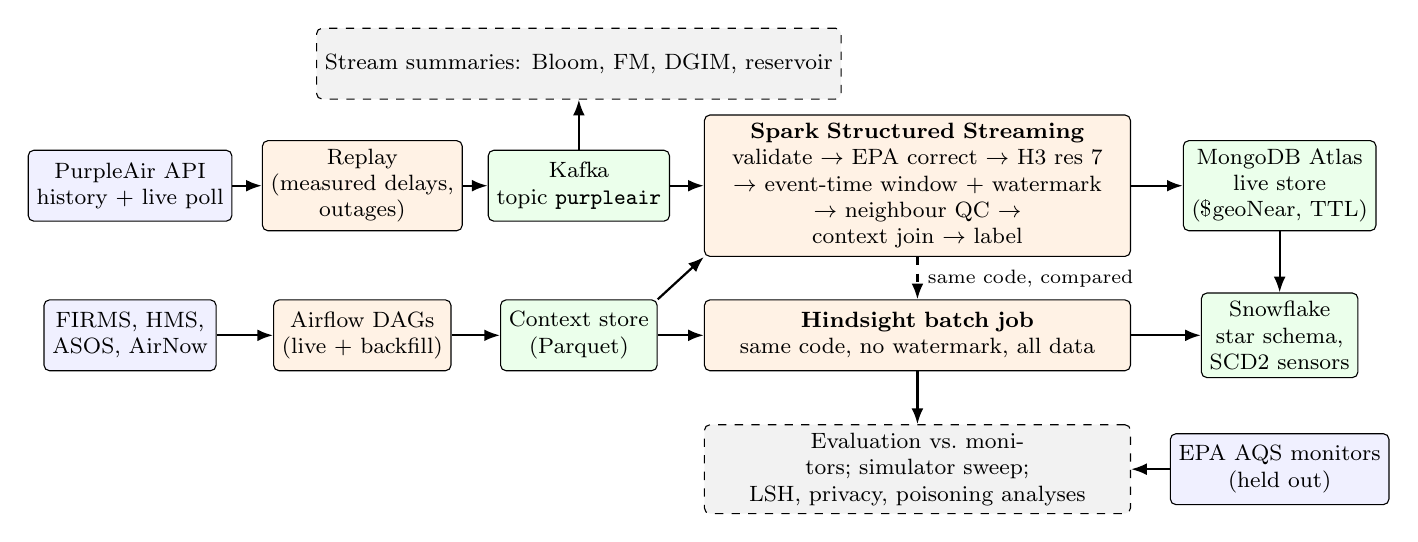
\begin{tikzpicture}[font=\footnotesize,
  box/.style={draw, rounded corners=2pt, align=center, minimum height=9mm, inner sep=3pt, fill=white},
  src/.style={box, fill=blue!6}, proc/.style={box, fill=orange!10}, store/.style={box, fill=green!8},
  side/.style={box, fill=gray!10, dashed}, arr/.style={-{Latex[length=2mm]}, thick}]
\node[side] (sum) at (5.7, 1.55) {Stream summaries: Bloom, FM, DGIM, reservoir};
\node[src] (pa) at (0, 0) {PurpleAir API\\history + live poll};
\node[proc] (replay) at (2.95, 0) {Replay\\(measured delays,\\outages)};
\node[store] (kafka) at (5.7, 0) {Kafka\\topic \texttt{purpleair}};
\node[proc, text width=52mm] (spark) at (10.0, 0) {\textbf{Spark Structured Streaming}\\validate $\rightarrow$ EPA correct $\rightarrow$ H3 res 7\\$\rightarrow$ event-time window + watermark\\$\rightarrow$ neighbour QC $\rightarrow$ context join $\rightarrow$ label};
\node[store] (mongo) at (14.6, 0) {MongoDB Atlas\\live store\\(\$geoNear, TTL)};
\node[src] (pub) at (0, -1.9) {FIRMS, HMS,\\ASOS, AirNow};
\node[proc] (airflow) at (2.95, -1.9) {Airflow DAGs\\(live + backfill)};
\node[store] (ctx) at (5.7, -1.9) {Context store\\(Parquet)};
\node[proc, text width=52mm] (batch) at (10.0, -1.9) {\textbf{Hindsight batch job}\\same code, no watermark, all data};
\node[store] (snow) at (14.6, -1.9) {Snowflake\\star schema,\\SCD2 sensors};
\node[side, text width=52mm] (eval) at (10.0, -3.6) {Evaluation vs.\ monitors; simulator sweep;\\LSH, privacy, poisoning analyses};
\node[src] (mon) at (14.6, -3.6) {EPA AQS monitors\\(held out)};
\draw[arr] (pa) -- (replay); \draw[arr] (replay) -- (kafka); \draw[arr] (kafka) -- (spark);
\draw[arr] (spark) -- (mongo); \draw[arr] (pub) -- (airflow); \draw[arr] (airflow) -- (ctx);
\draw[arr] (ctx.north east) -- (spark.south west);
\draw[arr] (kafka) -- (sum);
\draw[arr] (ctx) -- (batch);
\draw[arr, dashed] (spark) -- (batch) node[midway, right, font=\scriptsize]{same code, compared};
\draw[arr] (batch) -- (snow); \draw[arr] (mongo) -- (snow);
\draw[arr] (batch) -- (eval); \draw[arr] (mon) -- (eval);
\end{tikzpicture}
\caption{SmokeStream flow. Readings are replayed into Kafka with measured delays; Spark finalizes event-time windows under a watermark, checks each sensor against its neighbours, joins fire, plume and wind context published by Airflow, and labels elevated hexagons. Finalized windows go to the MongoDB live store and, with the hindsight baseline that runs the same code on complete data, to Snowflake. Stream summaries read the same Kafka stream; regulatory monitors are used only for evaluation.}
\label{fig:flow}
\end{figure*}

\subsection{Ingestion}
Each message carries the sensor index, event time, arrival time, location, both laser channels, PM\textsubscript{1} and relative humidity. The Kafka producer keys messages by sensor index, so one sensor's readings stay ordered within a partition; demo topics have four partitions. For experiments the same messages are written to one JSON-lines file per simulated minute, which Spark reads one file per micro-batch.

\subsection{Stream processing}
Both pipelines run the same PySpark code. Readings are validated (range checks; the two laser channels must agree within 5\ugm{} or 70\%) and corrected with the EPA U.S.-wide equation~\cite{barkjohn2021},
\begin{equation}
\text{PM}_{2.5} = \max\left(0,\; 0.524\,\overline{\text{PA}} - 0.0862\,\text{RH} + 5.75\right),
\end{equation}
where $\overline{\text{PA}}$ is the mean of the two channels and RH the relative humidity. Each reading is mapped to an H3 cell at resolution 7 (about 5\,km\textsuperscript{2}) and averaged per sensor in tumbling event-time windows. The streaming job declares a watermark of $w$ minutes, so a window is finalized once the maximum event time seen exceeds its end by $w$; the batch job sees every reading. The live job uses a 5-second processing-time trigger with checkpointing, and a \texttt{foreachBatch} sink appends finalized windows to Parquet and upserts them into MongoDB.

\subsection{Neighbour quality check}
For sensor $i$ in a window, let $m_i$ be the median of the other sensors within two hexagon rings (about 5\,km). The sensor is deviant when
\begin{equation}
|x_i - m_i| > 10\text{\ugm} \quad\text{and}\quad \frac{|x_i - m_i|}{\max(m_i, 5)} > 1,
\end{equation}
provided at least two neighbours report. It is excluded once it was deviant in at least 75\% of its informed windows over the last \emph{QC history} minutes (at least two windows). Short history removes faulty sensors quickly but can also suppress real local spikes and the leading edge of a smoke front.

\subsection{Context and labels}
Each elevated hexagon window (AQI above 100) receives four signals: \emph{extent} (the share of hexagons within three rings also elevated), the PM\textsubscript{1}/PM\textsubscript{2.5} ratio (fine particles dominate smoke), HMS plume overlap, and an upwind fire (within 150\,km and 45\textdegree{} of the upwind direction, or within 50\,km in calm air). Context counts only if it was published and picked up by a refresh at the configured interval before the decision time, the window end plus the watermark; this is how context freshness becomes a knob. A rule labels each window \emph{wildfire}, \emph{local} or \emph{uncertain}, and a smoke alert fires when AQI exceeds 150 and the label is not local.

\subsection{Live store}
Finalized windows are upserted into a MongoDB Atlas collection with one document per hexagon: H3 id, GeoJSON point, window bounds, PM\textsubscript{2.5}, AQI and category, label, alert flag and emission time. A unique index on the H3 id, a 2dsphere index for \$geoNear ``AQI near me'' queries and a 24-hour TTL index keep it small and current. Micro-batches can finish out of order, so the upsert replaces a document only with a later window.

\subsection{Warehouse}
A Snowflake~\cite{dageville2016} star schema (Table~\ref{tab:schema}) holds monitors, context, readings and every pipeline run side by side, so every stream-versus-hindsight comparison is a self-join on hexagon and window. The sensor dimension is a Type~2 slowly changing dimension: a sensor that moves gets its current row closed and a new version, and each reading joins the version valid at its time. Loads replace the slice they own (a season or a run), so reruns never duplicate rows, and the loader recomputes RQ1 in SQL and fails unless it matches the Python results; the same SQL runs in DuckDB in the test suite.

\begin{table}[t]
\caption{Warehouse star schema (Snowflake).}
\label{tab:schema}
\centering\scriptsize
\setlength{\tabcolsep}{3pt}
\begin{tabular}{>{\raggedright\arraybackslash}p{34mm}>{\raggedright\arraybackslash}p{48mm}}
\toprule
Table & Grain and role \\
\midrule
\texttt{DIM\_SENSOR} & sensor version (SCD Type 2: location, validity) \\
\texttt{DIM\_H3\_CELL} & H3 cell, resolution and center point \\
\texttt{DIM\_TIME} & 2-minute slot, UTC and local, season \\
\texttt{DIM\_PIPELINE\_CONFIG} & run and knob setting (mode, window, \dots) \\
\texttt{FACT\_READING} & one corrected reading with its QC flag \\
\texttt{FACT\_HEX\_WINDOW} & one hexagon window of one run and setting \\
\texttt{FACT\_ALERT} & hexagon windows that raised a smoke alert \\
\texttt{FACT\_MONITOR\_HOURLY} & monitor-hour of PM\textsubscript{2.5} (ground truth) \\
\texttt{FACT\_FIRE\_DETECTION} & fire detection with publication time \\
\texttt{FACT\_PLUME\_CELL} & H3 cell under an HMS plume, with validity \\
\texttt{FACT\_WIND\_OBS} & airport wind observation \\
\bottomrule
\end{tabular}
\end{table}

\subsection{Orchestration}
Six Airflow DAGs (Table~\ref{tab:dags}) run in their own environment and call project scripts, so Airflow and Spark never share packages. The live feeds merge each fetch into one file per day and keep the time a record was first fetched as its publication time, so live data obeys the same freshness rules as the replays. Their schedules are the live counterpart of the context-refresh knob.

\begin{table}[t]
\caption{Airflow DAGs.}
\label{tab:dags}
\centering\scriptsize
\setlength{\tabcolsep}{3pt}
\begin{tabular}{>{\raggedright\arraybackslash}p{36mm}>{\raggedright\arraybackslash}p{11mm}>{\raggedright\arraybackslash}p{33mm}}
\toprule
DAG & Schedule & Source and output \\
\midrule
\texttt{ingest\_fire\_detections} & 30 min & FIRMS near-real-time VIIRS fires \\
\texttt{ingest\_smoke\_plumes} & 3 h & HMS plumes as H3 cells \\
\texttt{ingest\_weather} & 1 h & ASOS airport wind \\
\texttt{ingest\_monitors} & hourly & AirNow PM\textsubscript{2.5} (evaluation only) \\
\texttt{backfill\_fire\_seasons} & manual & AQS, FIRMS, HMS, ASOS archives \\
\texttt{load\_snowflake} & daily & setup, load, verify against Python \\
\bottomrule
\end{tabular}
\end{table}

\section{Methodology}
\subsection{A validated simulator of watermark semantics}
Replaying a 60-day season through the engine in 1-minute micro-batches took about 0.27\,s per batch, or 6.5 hours per configuration, which rules out a sweep of dozens of configurations. We therefore simulate the engine. Records are grouped into the same arrival slices the replay produces; for slice $k$ let $W_k = \max e - w$ over all records seen through slice $k$. A window is finalized in the first slice whose $W_k$ reaches its end, and a record in slice $k$ is dropped as late only if its window ended at or before $W_{k-1}$.

That last rule was not our first guess. Our first version used $W_k$, and an automated test that runs Spark and the simulator on the same replay and compares every window failed: the engine counted readings the simulator had dropped. Spark (since 3.4) filters late rows with the previous batch's watermark and evicts state with the current one. With the corrected rule the outputs match exactly, including neighbour exclusions carried across batches, context features and labels. A second pitfall concerns batch granularity: Spark judges lateness once per micro-batch, so if each batch spans hours of data no reading is ever late and every watermark setting produces identical output. Replays must slice batches in simulated time, not wall-clock time.

\subsection{Evaluation}
Every configuration is compared with the hindsight baseline at the same window size (RMSE, coverage, label agreement) and with held-out monitors. For monitor $s$ and hour $h$, PM\textsubscript{2.5} is estimated from the hexagon windows $c$ within 5\,km,
\begin{equation}
\hat y_{s,h} = \frac{\sum_c w_{s,c}\, x_{c,h}}{\sum_c w_{s,c}}, \qquad w_{s,c} = \max(d_{s,c}, 0.5\,\text{km})^{-2},
\end{equation}
giving RMSE, bias and $R^2$, and, on Unhealthy hours (above 55.4\ugm), alert precision, recall and false-alarm rate. For each Unhealthy episode, the lead time is
\begin{equation}
L = (h_{\text{onset}} + 1\,\text{h} + 30\,\text{min}) - t_{\text{first alert}},
\end{equation}
the time between the stream's first nearby alert and when the official hourly value would have been posted. For RQ3, two people label a stratified sample of elevated events as wildfire, local or uncertain, blind to the pipeline's labels; agreement is measured with Cohen's kappa.

\subsection{Experiment design}
Window 10, 30 and 60 minutes; watermark 0, 5 and 15 minutes; QC history 30, 120 and 360 minutes; context refresh 15, 60 and 360 minutes. Each knob is varied around the default (10, 5, 120, 60), with watermark and QC history crossed: 13 settings per run, each scored against its own hindsight baseline and the monitors.

\subsection{Stream summaries}
On the 2020 replay in arrival order we deliver 2\% of messages a second time, up to 10 minutes later, as Kafka's at-least-once delivery does after producer retries or consumer restarts, and compare each summary with an exact computation.
\emph{Bloom filter}~\cite{bloom1970}: keyed on (sensor, event time); for capacity $n$ and target false-positive rate $p$ it uses
\begin{equation}
m = \left\lceil -\frac{n \ln p}{(\ln 2)^2} \right\rceil \text{ bits}, \qquad k = \frac{m}{n}\ln 2 \text{ hashes}.
\end{equation}
Two filters rotate every hour, so a key is remembered for one to two hours, longer than any redelivery. \emph{Flajolet--Martin}~\cite{flajolet1985}: for each of 64 hash functions a bitmap of observed trailing-zero counts; with $R_j$ its lowest unset bit, the distinct count is estimated as $2^{\bar R}/0.77351$, taking the median over 8 groups of the mean $R_j$. \emph{DGIM}~\cite{datar2002}: buckets of power-of-two sizes, at most two per size, count the 1s (readings above 35.4\ugm) among the last $N$ readings within 50\% in $O(\log^2 N)$ bits. \emph{Reservoir sampling}~\cite{vitter1985}: after $t$ items each is kept with probability $k/t$; we sample $k=50$ Unhealthy readings, the stream labelers would draw from, over 1,000 seeds.

\subsection{Locality-sensitive hashing}
Each sensor-day becomes a 144-slot curve of corrected PM\textsubscript{2.5}, log-scaled and z-normalized, so the cosine similarity of two curves is their Pearson correlation $\rho$. SimHash~\cite{charikar2002} draws random hyperplanes; two curves at angle $\theta = \arccos\rho$ agree on one bit with probability $1-\theta/\pi$. With $b=16$ bands of $r=8$ bits, a pair becomes a candidate with probability
\begin{equation}
P(\rho) = 1 - \left(1 - (1 - \arccos(\rho)/\pi)^{r}\right)^{b},
\end{equation}
0.94 at $\rho=0.8$ and 0.23 at $\rho=0.3$. Candidates are verified exactly at $\rho\ge0.8$. A sensor's \emph{coherence} is the share of the other sensors on the same day it moves with; regional smoke should raise it.

\subsection{Privacy}
A hexagon with one sensor publishes one household's readings. For hourly hexagon means we apply (a) k-anonymity by generalization~\cite{sweeney2002}: publish at resolution 7 only if $k$ distinct sensors contribute, otherwise at the parent cell (resolution 6, then 5) once it has $k$, otherwise suppress; and (b) the Laplace mechanism~\cite{dwork2006}. Each sensor's hourly value is clipped to $[0, C]$, so replacing one sensor changes the mean of $n$ sensors by at most $C/n$, and the published value is
\begin{equation}
\tilde x = \bar x + \text{Lap}\!\left(\frac{C}{n\,\varepsilon}\right).
\end{equation}
$\varepsilon$ is per hourly release; a day of releases composes to $24\varepsilon$. Utility is measured against the non-private resolution-7 means: RMSE and agreement on the AQI-above-100 flag, averaged over 10 noise seeds.

\subsection{Data poisoning}
Into the July 2021 window we inject fake sensors that report a steady, plausible 120\ugm{} (AQI 184) for 24 hours with both channels in agreement, so the channel check cannot catch them: four \emph{lone} fakes, each in the hexagon of a different honest sensor, and three \emph{colluding} fakes in one hexagon (a Sybil attack~\cite{douceur2002}). We run the hindsight pipeline with the neighbour check on and off and count false Unhealthy hexagon-windows.

\section{Results}
\subsection{RQ1: the cost of real time}
Under the measured delay profile, the 2020 stream missed 2.0--2.1\% of readings. With 10-minute windows, streaming hexagon values differed from full hindsight by an RMSE of 0.11--0.12\ugm{} (0.6\ugm{} with 30- or 60-minute windows), about 150 times smaller than the error of sensors against monitors (17.4\ugm). The partial delay profile we used for the status report gave the same picture. Against monitors, 2020 smoke alerts were 88\% precise with a 2\% false-alarm rate and caught 54\% of Unhealthy monitor-hours (sensor coverage, not latency, limits recall); they arrived a median 99 minutes before the official hourly value, against 120 minutes for the hindsight baseline. The event windows agree: late-data RMSE was 0.18--0.61\ugm.

\begin{table*}[t]
\caption{All 13 settings on the 2020 season (measured delay profile). Latency: window plus median wait until the watermark closes it. Missed: readings dropped as late. RMSE and labels are against the hindsight baseline at the same window; alerts and lead time are against held-out monitors (14,724 monitor-hours at 20 sites).}
\label{tab:sweep}
\centering\footnotesize
\begin{tabular}{rrrrrrrrrrr}
\toprule
Window & Watermark & QC hist. & Context & Latency & Missed & RMSE vs. & Label & Smoke-alert & Smoke-alert & Lead \\
(min) & (min) & (min) & (min) & (min) & (\%) & hindsight & agreement & precision & recall & (min) \\
\midrule
10 & 5 & 120 & 60 & 31 & 2.0 & 0.122 & 90.6\% & 0.884 & 0.541 & 99 \\
30 & 5 & 120 & 60 & 51 & 2.0 & 0.603 & 92.6\% & 0.886 & 0.542 & 69 \\
60 & 5 & 120 & 60 & 81 & 2.0 & 0.588 & 93.7\% & 0.884 & 0.541 & 69 \\
10 & 0 & 120 & 60 & 21 & 2.1 & 0.122 & 90.6\% & 0.884 & 0.541 & 109 \\
10 & 15 & 120 & 60 & 41 & 2.0 & 0.122 & 91.1\% & 0.884 & 0.541 & 89 \\
10 & 5 & 30 & 60 & 31 & 2.0 & 0.107 & 90.6\% & 0.884 & 0.541 & 99 \\
10 & 5 & 360 & 60 & 31 & 2.0 & 0.114 & 90.6\% & 0.884 & 0.541 & 99 \\
10 & 5 & 120 & 15 & 31 & 2.0 & 0.122 & 92.3\% & 0.884 & 0.541 & 99 \\
10 & 5 & 120 & 360 & 31 & 2.0 & 0.122 & 84.1\% & 0.884 & 0.541 & 99 \\
10 & 0 & 30 & 60 & 21 & 2.1 & 0.107 & 90.6\% & 0.884 & 0.541 & 109 \\
10 & 0 & 360 & 60 & 21 & 2.1 & 0.114 & 90.6\% & 0.884 & 0.541 & 109 \\
10 & 15 & 30 & 60 & 41 & 2.0 & 0.106 & 91.1\% & 0.884 & 0.541 & 89 \\
10 & 15 & 360 & 60 & 41 & 2.0 & 0.114 & 91.1\% & 0.884 & 0.541 & 89 \\
\bottomrule
\end{tabular}
\end{table*}

\subsection{RQ2: the frontier}
Fig.~\ref{fig:frontier} shows accuracy against decision latency. The watermark moves latency by 10 minutes per step without changing accuracy (0.122\ugm{} at 0, 5 or 15 minutes in 2020): readings are rarely later than the median 80\,s delay, so a short watermark is almost free and every extra minute of waiting buys nothing. Longer windows add 20--50 minutes and do not consistently bring the stream closer to hindsight (0.60 vs.\ 0.12\ugm{} in 2020, 0.18 vs.\ 0.61\ugm{} in the 2021 smoke). QC history barely matters (0.107--0.122\ugm). \textbf{Context freshness is the knob that matters} (Fig.~\ref{fig:context}): with 6-hour refreshes instead of 15 minutes, label agreement with hindsight fell from 92.3\% to 84.1\% in 2020, from 87.7\% to 84.4\% in the 2021 smoke, and from 100\% to 55\% in the July 2021 window. Lead time follows the watermark: 109, 99 and 89 minutes at 0, 5 and 15 minutes.

\begin{figure}[t]
\centering
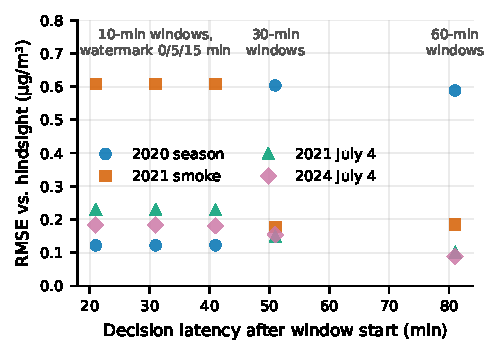
\includegraphics[width=\columnwidth]{frontier}
\caption{Accuracy against latency. Each point is one setting; decision latency is the window length plus the median wait after the window ends until the watermark closes it, which includes waiting for the next 10-minute reading. All settings stay within 0.61\ugm{} of hindsight, far below the 17.4\ugm{} sensor-to-monitor error.}
\label{fig:frontier}
\end{figure}

\begin{figure}[t]
\centering
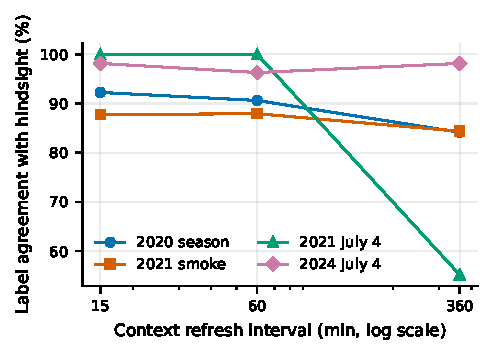
\includegraphics[width=\columnwidth]{context_refresh}
\caption{Label agreement with hindsight as fire and plume context gets staler (10-minute windows, 5-minute watermark).}
\label{fig:context}
\end{figure}

\subsection{RQ3: smoke or fireworks? (preliminary)}
On the two July 4 windows the pipeline behaved very differently. In 2021, 15 of 16 elevated events were labeled \emph{uncertain}: sparse sensors gave no extent signal either way. In 2024, 13 of 14 were labeled \emph{wildfire}: fire detections and plumes elsewhere in the region made fireworks look like smoke, the failure mode we anticipated for sparse sensor areas. In the 2021 smoke window, alerts caught 88\% of Unhealthy monitor-hours, a median 169 minutes early, but only 49\% were precise. Blind hand labels of these 100 events by two labelers (Cohen's kappa) are in progress; until then these counts are pipeline labels, not accuracy.

\begin{table}[t]
\caption{Event windows at the default setting (10-minute window, 5-minute watermark). Label agreement with hindsight at three context-refresh intervals; smoke alerts against monitors.}
\label{tab:windows}
\centering\footnotesize
\setlength{\tabcolsep}{2.5pt}
\begin{tabular}{lrrrrrrr}
\toprule
 & RMSE vs. & \multicolumn{3}{c}{Label agreement (\%)} & Alert & Alert & Lead \\
Window & hindsight & 15 min & 60 min & 6 h & prec. & recall & (min) \\
\midrule
July 4, 2021 & 0.228 & 100.0 & 100.0 & 55.2 & 1.00 & 0.17 & 39 \\
Caldor smoke & 0.607 & 87.7 & 87.9 & 84.4 & 0.49 & 0.88 & 169 \\
July 4, 2024 & 0.183 & 98.1 & 96.3 & 98.1 & 1.00 & 0.33 & 69 \\
\bottomrule
\end{tabular}
\end{table}

\subsection{RQ4: performance}\label{sec:rq4}
On one laptop, Kafka and Spark sustained 641 messages/s at 300$\times$ real time on synthetic load with 95th-percentile end-to-end latency of 11.5\,s, and drained a backlog at about 14,500 messages/s. On real data, replaying 14 hours of the September 10--11, 2020 smoke at 120$\times$ through Kafka, Spark and MongoDB Atlas put all 2,411 windows into the live store with a median latency of 16.4\,s (95th percentile 17.2\,s). Of that, 9.5\,s is \emph{designed} waiting, the 19 simulated minutes a window waits for later readings to pass the watermark, and about 7\,s is the system: the 5-second trigger, processing and the Atlas write. The simulator replaced 6.5 hours per configuration with seconds.

\begin{figure}[t]
\centering
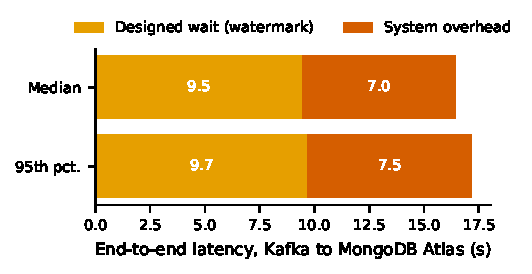
\includegraphics[width=\columnwidth]{latency_split}
\caption{Where real-data latency goes (14 hours of September 2020 at 120$\times$, 2,411 windows). The designed wait is the time a window waits for later readings to pass the watermark, converted to wall-clock seconds; the rest is the trigger, processing and the MongoDB Atlas write.}
\label{fig:latency}
\end{figure}

\subsection{Stream summaries}\label{sec:sketchres}
Table~\ref{tab:sketch} compares each summary with the exact answer on 145,017 deliveries. The rotating Bloom filter caught all 2,843 duplicate deliveries (no false negatives, by construction) and wrongly dropped 7 unique readings (0.005\%), at 14.4 bits per key instead of 128. Flajolet--Martin counted active sensors per hour within 3.4\% on average in 256 bytes; DGIM stayed within its 50\% bound and used 52 bytes instead of 1,250 for a 10,000-reading window. The reservoir kept each tenth of the stream 9.8--10.3\% of the time (ideal 10\%), so a labeling sample drawn as events arrive is unbiased toward early or late events. At our sample size an exact set would also fit in memory; the summaries keep fixed memory as the network grows to tens of thousands of sensors. Fig.~\ref{fig:dgim} follows DGIM across the season: it tracks the exact count through the September smoke, and the sawtooth comes from counting the oldest bucket as half.

\begin{figure}[t]
\centering
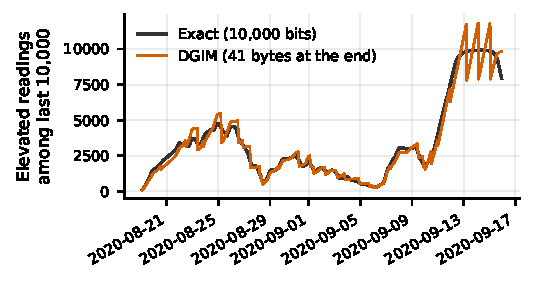
\includegraphics[width=\columnwidth]{dgim}
\caption{DGIM estimate against the exact count of readings above 35.4\ugm{} among the last 10,000, over the 2020 replay.}
\label{fig:dgim}
\end{figure}

\begin{table}[t]
\caption{Stream summaries against exact answers (2020 replay).}
\label{tab:sketch}
\centering\footnotesize
\setlength{\tabcolsep}{3pt}
\begin{tabular}{p{17mm}p{30mm}rr}
\toprule
Summary & Task & Error & Memory \\
\midrule
Bloom (rotating) & drop 2,843 duplicates & 0 missed, 7 false & 1.4\,KB \\
Flajolet--Martin & distinct sensors per hour & 3.4\% (p90 8.3\%) & 256\,B \\
DGIM, $N$=1,000 & elevated readings in last $N$ & 11.6\% (max 50\%) & $\le$30\,B \\
DGIM, $N$=10,000 & elevated readings in last $N$ & 10.9\% (max 43\%) & $\le$52\,B \\
Reservoir, $k$=50 & uniform event sample & $\pm$0.34 pp per decile & 50 items \\
\bottomrule
\end{tabular}
\end{table}

\subsection{LSH: which sensors move together}\label{sec:lshres}
Within each of 39 days, SimHash found 98.8\% of sensor pairs correlated above 0.8. Pooling all 1,025 sensor-days (524,800 pairs), it proposed 23.9\% of pairs as candidates and still found 98.2\% of the 16,246 similar pairs, a four-fold cut in comparisons that grows with the network. Coherence separates regional smoke from clean air on average: 0.28 on smoke days against 0.13 on clean days and 0.17 on moderate days, but the spread is wide (standard deviation 0.17). July 4 split: 0.29 in 2021, like a smoke day, because fireworks happen everywhere at once, and 0.10 in 2024. Coherence is a useful extra signal for RQ3, not a classifier on its own.

\begin{figure}[t]
\centering
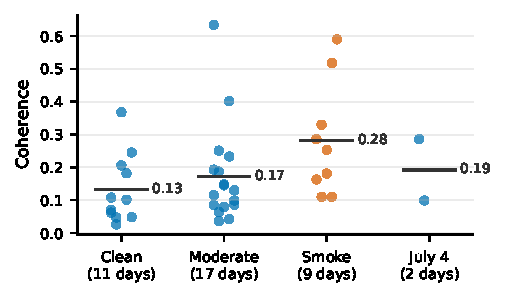
\includegraphics[width=\columnwidth]{coherence}
\caption{Coherence per day (share of other sensors moving together, correlation at least 0.8), by day type. Bars are means.}
\label{fig:coherence}
\end{figure}

\subsection{Privacy: what safe publishing costs}\label{sec:privres}
Our sensors are sparse: only 3.7\% of hexagon-hours at resolution 7 have two or more sensors. k-anonymity therefore forces generalization: with $k=3$, 48\% of hexagon-hours can be published (all at resolution 6 or 5) and AQI-above-100 alerts keep 93--94\% precision and recall; with $k=5$ only 11\% can. Differential privacy with the conservative clip $C=500$\ugm{} is unusable at these sizes (RMSE above 150\ugm{} at $\varepsilon=1$). Clipping instead at $C=100$\ugm{}, all an AQI-100 alert needs, makes it workable (Fig.~\ref{fig:privacy}): with $k=3$, $\varepsilon=2$ per hourly release keeps 87\% of alerts at 74\% precision, and $k=5$ keeps 90\% at 81\%. Privacy for a sparse network is bought with coverage and coarser cells; clipping to the decision threshold is the cheapest lever.

\begin{table}[t]
\caption{Privacy against utility on 20,139 hexagon-hours (2020, $C = 100$\ugm, 10 seeds). Published: share of hexagon-hours released; P/R: precision and recall of the AQI-above-100 flag against the non-private values.}
\label{tab:privacy}
\centering\scriptsize
\setlength{\tabcolsep}{2.5pt}
\begin{tabular}{rrrrrrr}
\toprule
$k$ & Published & No noise & $\varepsilon = 10$ & $\varepsilon = 2$ & $\varepsilon = 1$ \\
 & & P / R & P / R & P / R & P / R \\
\midrule
1 & 100\% & 1.00 / 1.00 & 0.84 / 0.92 & 0.54 / 0.74 & 0.46 / 0.65 \\
2 & 63\% & 0.94 / 0.95 & 0.90 / 0.93 & 0.68 / 0.84 & 0.56 / 0.76 \\
3 & 48\% & 0.93 / 0.94 & 0.91 / 0.93 & 0.74 / 0.87 & 0.62 / 0.79 \\
5 & 11\% & 0.94 / 0.94 & 0.93 / 0.94 & 0.81 / 0.90 & 0.69 / 0.84 \\
\bottomrule
\end{tabular}
\end{table}

\begin{figure}[t]
\centering
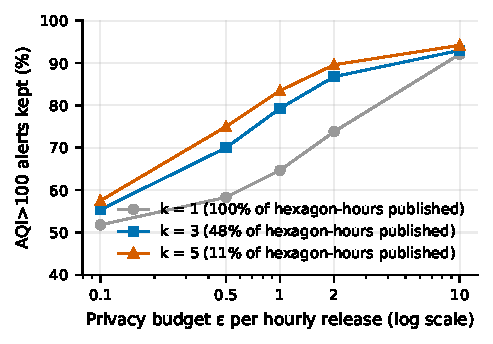
\includegraphics[width=\columnwidth]{privacy}
\caption{Alerts kept under k-anonymity plus the Laplace mechanism (2020, values clipped at 100\ugm). Larger $k$ means fewer, coarser published cells but less noise per cell.}
\label{fig:privacy}
\end{figure}

\subsection{Poisoning: can fake sensors raise alerts?}\label{sec:poisonres}
Without the neighbour check, four lone fakes produced 438 false Unhealthy hexagon-windows in 24 hours. With it, three of the four were excluded within one or two windows (at most one false alert each); the fourth had only one honest sensor within two rings, below the two-neighbour minimum, and alerted all 144 windows (146 in total). Three colluding fakes in one hexagon alerted in all 144 windows with or without the check: they are each other's neighbours, so the median they are compared to is their own value. The check stops faulty sensors where the network is dense, but not a Sybil attack or a lone fake in a sparse area; defenses would weigh sensor age and history, limit how much one owner's sensors can count, and cross-check satellite plumes and monitors.

\begin{table}[t]
\caption{False Unhealthy hexagon-windows in 24 hours (July 2021 window; 0 in the clean run).}
\label{tab:poison}
\centering\footnotesize
\begin{tabular}{lrrr}
\toprule
Scenario & Fakes & Check off & Check on \\
\midrule
Lone, $\ge$2 honest neighbours & 3 & 294 & 2 \\
Lone, 1 honest neighbour & 1 & 144 & 144 \\
Colluding, one hexagon & 3 & 144 & 144 \\
\bottomrule
\end{tabular}
\end{table}

\section{Discussion and Threats to Validity}
\textbf{Delay profile.} About 18 hours of live polling over 31 hours; the median matched an earlier partial profile (80 vs.\ 82\,s), but night hours are under-sampled. \textbf{Context timing.} Archived fire and plume records lack publication times; we assume typical delays (3 hours for FIRMS, 2 hours after an HMS plume ends). \textbf{Ground truth.} Monitors are sparse and hourly, and near-fire monitors dominate squared errors. \textbf{Sample.} Points-based API pricing limits each window to a few dozen sensors; sparsity drives the RQ3, privacy and poisoning findings, and a denser network would change them, probably for the better. \textbf{Labels.} The labeling rule is deliberately simple and untuned, and RQ3 is preliminary until the hand labels are scored. \textbf{Simulator scope.} The simulator reproduces Spark's semantics for the file-sliced replay; the engine remains the reference for performance.

\subsection*{Recommendations for practitioners}
Our results suggest a few settings for anyone building a real-time map from crowdsourced sensors. Keep the watermark short (a few minutes, a little above the typical arrival delay): it buys almost no accuracy, while every extra minute delays every alert. Refresh slow context sources as often as they publish; on our data the refresh interval moved label agreement by up to 45 points while the watermark moved it by under one. Sample or recruit sensors around regulatory monitors so the system can be checked against ground truth. When privacy matters, generalize sparse cells to a coarser resolution and clip values at the decision threshold before adding noise. Treat the neighbour check as a defense against faulty sensors, not malicious ones.

\section{Responsible Use}
A smoke map is a public-health tool, so its errors have costs on both sides: a missed alert leaves people outdoors in unhealthy air, and repeated false alarms teach them to ignore the next one. We report both precision and recall and state where coverage, not latency, limits recall. Sensor hosts are private households; we publish hexagon aggregates, never sensor coordinates or raw readings, and Section~\ref{sec:privres} quantifies what stronger protections cost. Because anyone can register a sensor, we tested the quality check against fake devices and report where it fails. PurpleAir's terms do not allow redistributing raw readings, so we release code, sensor IDs and time ranges instead. Coverage is uneven: even with sensors sampled around monitors, only 16 of 20 monitors had a sensor within 5\,km, and areas without sensors get no alert at all, so a real deployment should show where it cannot see.

\section{Lessons Learned and Best Practices}\label{sec:lessons}
\begin{itemize}
\item \textbf{Test the engine, not the documentation.} An automated equivalence test between Spark and our simulator exposed that late rows are filtered with the previous batch's watermark. Without it every RQ2 number would have been subtly wrong.
\item \textbf{Control micro-batch size in simulated time.} Large replay batches silently make every watermark setting identical.
\item \textbf{Measure the inputs that shape the result.} We measured arrival delays from the live network instead of assuming them, and re-validated the sensor correction against monitors; the ``extended'' correction in public tools would have inflated smoke by up to two thirds.
\item \textbf{Freshness of context beats waiting for data.} The most expensive knob was not the watermark but how often slow sources are refreshed, which is an orchestration (Airflow) decision.
\item \textbf{Make warehouse loads idempotent and self-checking.} Replace-by-slice loads and a SQL re-computation of RQ1 that must match the Python results caught type and null issues before they reached the report.
\item \textbf{Budget paid APIs like compute.} Estimating cost before every download, capping spend and measuring the real price per row (4 points plus 2 per request) let us add three event windows within the free allowance.
\item \textbf{Sparse networks change everything downstream.} Coverage limited alert recall, the extent signal, privacy and poisoning defense alike; sampling sensors around monitors was the single most useful data decision.
\end{itemize}

\section{Conclusion and Future Work}\label{sec:conclusion}
Real time is cheap where engineers worry most and expensive where they look least: with arrival delays measured from the live network, late data costs a fraction of a microgram, while stale fire and plume context costs up to 45 points of label agreement. Smoke alerts can arrive about an hour and a half before official values. Next steps are scoring RQ3 with two labelers, denser sensor samples for 2021 and 2024, sensitivity to faster and slower delay profiles, and a Sybil-resistant quality check. We plan to submit the measurement methodology and frontier to a workshop at ACM DEBS or ACM SIGSPATIAL.

\section*{Data and Code Availability}
Code, the delay profile, sensor IDs, time ranges and analysis outputs are at \url{https://github.com/VRAJ8/smokestream}. PurpleAir's terms do not allow redistributing raw readings; others re-download them with their own key. All other data is public.

\section*{Contributions (CRediT)}
% Fill in names and shares. Roles from the CRediT taxonomy (credit.niso.org).
Conceptualization: [name, \%]. Methodology: [name, \%]. Software: [name, \%]. Validation: [name, \%]. Formal analysis: [name, \%]. Investigation: [name, \%]. Data curation: [name, \%]. Writing -- original draft: [name, \%]. Writing -- review \& editing: [name, \%]. Visualization: [name, \%]. Project administration: [name, \%].

\section*{Use of Generative AI and Other Sources}
% To be written by the authors.
[To be completed by the authors.]

\bibliographystyle{IEEEtran}
\begin{thebibliography}{99}
\bibitem{reid2016} C. E. Reid, M. Brauer, F. H. Johnston, M. Jerrett, J. R. Balmes, and C. T. Elliott, ``Critical review of health impacts of wildfire smoke exposure,'' \emph{Environ. Health Perspect.}, vol. 124, no. 9, pp. 1334--1343, 2016.
\bibitem{burke2021} M. Burke, A. Driscoll, S. Heft-Neal, J. Xue, J. Burney, and M. Wara, ``The changing risk and burden of wildfire in the United States,'' \emph{Proc. Natl. Acad. Sci.}, vol. 118, no. 2, e2011048118, 2021.
\bibitem{burke2023} M. Burke, M. L. Childs, B. de la Cuesta, M. Qiu, J. Li, C. F. Gould, S. Heft-Neal, and M. Wara, ``The contribution of wildfire to PM2.5 trends in the USA,'' \emph{Nature}, vol. 622, pp. 761--766, 2023.
\bibitem{childs2022} M. L. Childs \emph{et al.}, ``Daily local-level estimates of ambient wildfire smoke PM2.5 for the contiguous US,'' \emph{Environ. Sci. Technol.}, vol. 56, no. 19, pp. 13607--13621, 2022.
\bibitem{bi2020} J. Bi, A. Wildani, H. H. Chang, and Y. Liu, ``Incorporating low-cost sensor measurements into high-resolution PM2.5 modeling at a large spatial scale,'' \emph{Environ. Sci. Technol.}, vol. 54, no. 4, pp. 2152--2162, 2020.
\bibitem{schroeder2014} W. Schroeder, P. Oliva, L. Giglio, and I. A. Csiszar, ``The New VIIRS 375\,m active fire detection data product: Algorithm description and initial assessment,'' \emph{Remote Sens. Environ.}, vol. 143, pp. 85--96, 2014.
\bibitem{rolph2009} G. D. Rolph \emph{et al.}, ``Description and verification of the NOAA smoke forecasting system: The 2007 fire season,'' \emph{Weather Forecast.}, vol. 24, no. 2, pp. 361--378, 2009.
\bibitem{firemap} U.S. EPA and USDA Forest Service, ``AirNow Fire and Smoke Map.'' [Online]. Available: \url{https://fire.airnow.gov}
\bibitem{holder2020} A. L. Holder \emph{et al.}, ``Field evaluation of low-cost particulate matter sensors for measuring wildfire smoke,'' \emph{Sensors}, vol. 20, no. 17, 4796, 2020.
\bibitem{delp2020} W. W. Delp and B. C. Singer, ``Wildfire smoke adjustment factors for low-cost and professional PM2.5 monitors with optical sensors,'' \emph{Sensors}, vol. 20, no. 13, 3683, 2020.
\bibitem{barkjohn2021} K. K. Barkjohn, B. Gantt, and A. L. Clements, ``Development and application of a United States-wide correction for PM2.5 data collected with the PurpleAir sensor,'' \emph{Atmos. Meas. Tech.}, vol. 14, pp. 4617--4637, 2021.
\bibitem{barkjohn2022} K. K. Barkjohn \emph{et al.}, ``Correction and accuracy of PurpleAir PM2.5 measurements for extreme wildfire smoke,'' \emph{Sensors}, vol. 22, no. 24, 9669, 2022.
\bibitem{liang2021} Y. Liang, D. Sengupta, M. J. Campmier, D. M. Lunderberg, J. S. Apte, and A. H. Goldstein, ``Wildfire smoke impacts on indoor air quality assessed using crowdsourced data in California,'' \emph{Proc. Natl. Acad. Sci.}, vol. 118, no. 36, e2106478118, 2021.
\bibitem{kreps2011} J. Kreps, N. Narkhede, and J. Rao, ``Kafka: A distributed messaging system for log processing,'' in \emph{Proc. NetDB Workshop}, 2011.
\bibitem{armbrust2018} M. Armbrust \emph{et al.}, ``Structured Streaming: A declarative API for real-time applications in Apache Spark,'' in \emph{Proc. ACM SIGMOD}, 2018, pp. 601--613.
\bibitem{zaharia2013} M. Zaharia, T. Das, H. Li, T. Hunter, S. Shenker, and I. Stoica, ``Discretized streams: Fault-tolerant streaming computation at scale,'' in \emph{Proc. ACM SOSP}, 2013, pp. 423--438.
\bibitem{carbone2015} P. Carbone, A. Katsifodimos, S. Ewen, V. Markl, S. Haridi, and K. Tzoumas, ``Apache Flink: Stream and batch processing in a single engine,'' \emph{IEEE Data Eng. Bull.}, vol. 38, no. 4, pp. 28--38, 2015.
\bibitem{akidau2013} T. Akidau \emph{et al.}, ``MillWheel: Fault-tolerant stream processing at internet scale,'' \emph{Proc. VLDB Endow.}, vol. 6, no. 11, pp. 1033--1044, 2013.
\bibitem{akidau2015dataflow} T. Akidau \emph{et al.}, ``The Dataflow model: A practical approach to balancing correctness, latency, and cost in massive-scale, unbounded, out-of-order data processing,'' \emph{Proc. VLDB Endow.}, vol. 8, no. 12, pp. 1792--1803, 2015.
\bibitem{marz2015} N. Marz and J. Warren, \emph{Big Data: Principles and Best Practices of Scalable Realtime Data Systems}. Shelter Island, NY, USA: Manning, 2015.
\bibitem{kreps2014} J. Kreps, ``Questioning the Lambda architecture,'' O'Reilly Radar, 2014.
\bibitem{chintapalli2016} S. Chintapalli \emph{et al.}, ``Benchmarking streaming computation engines: Storm, Flink and Spark Streaming,'' in \emph{Proc. IEEE IPDPSW}, 2016, pp. 1789--1792.
\bibitem{karimov2018} J. Karimov, T. Rabl, A. Katsifodimos, R. Samarev, H. Heiskanen, and V. Markl, ``Benchmarking distributed stream data processing systems,'' in \emph{Proc. IEEE ICDE}, 2018, pp. 1507--1518.
\bibitem{leskovec2020} J. Leskovec, A. Rajaraman, and J. D. Ullman, \emph{Mining of Massive Datasets}, 3rd ed. Cambridge, U.K.: Cambridge Univ. Press, 2020.
\bibitem{bloom1970} B. H. Bloom, ``Space/time trade-offs in hash coding with allowable errors,'' \emph{Commun. ACM}, vol. 13, no. 7, pp. 422--426, 1970.
\bibitem{flajolet1985} P. Flajolet and G. N. Martin, ``Probabilistic counting algorithms for data base applications,'' \emph{J. Comput. Syst. Sci.}, vol. 31, no. 2, pp. 182--209, 1985.
\bibitem{datar2002} M. Datar, A. Gionis, P. Indyk, and R. Motwani, ``Maintaining stream statistics over sliding windows,'' \emph{SIAM J. Comput.}, vol. 31, no. 6, pp. 1794--1813, 2002.
\bibitem{vitter1985} J. S. Vitter, ``Random sampling with a reservoir,'' \emph{ACM Trans. Math. Softw.}, vol. 11, no. 1, pp. 37--57, 1985.
\bibitem{indyk1998} P. Indyk and R. Motwani, ``Approximate nearest neighbors: Towards removing the curse of dimensionality,'' in \emph{Proc. ACM STOC}, 1998, pp. 604--613.
\bibitem{charikar2002} M. S. Charikar, ``Similarity estimation techniques from rounding algorithms,'' in \emph{Proc. ACM STOC}, 2002, pp. 380--388.
\bibitem{sweeney2002} L. Sweeney, ``k-anonymity: A model for protecting privacy,'' \emph{Int. J. Uncertain. Fuzziness Knowl.-Based Syst.}, vol. 10, no. 5, pp. 557--570, 2002.
\bibitem{machanavajjhala2007} A. Machanavajjhala, D. Kifer, J. Gehrke, and M. Venkitasubramaniam, ``l-diversity: Privacy beyond k-anonymity,'' \emph{ACM Trans. Knowl. Discov. Data}, vol. 1, no. 1, 2007.
\bibitem{dwork2006} C. Dwork, F. McSherry, K. Nissim, and A. Smith, ``Calibrating noise to sensitivity in private data analysis,'' in \emph{Proc. Theory of Cryptography Conf. (TCC)}, 2006, pp. 265--284.
\bibitem{dwork2014} C. Dwork and A. Roth, ``The algorithmic foundations of differential privacy,'' \emph{Found. Trends Theor. Comput. Sci.}, vol. 9, no. 3--4, pp. 211--407, 2014.
\bibitem{biggio2012} B. Biggio, B. Nelson, and P. Laskov, ``Poisoning attacks against support vector machines,'' in \emph{Proc. ICML}, 2012, pp. 1467--1474.
\bibitem{douceur2002} J. R. Douceur, ``The Sybil attack,'' in \emph{Proc. Int. Workshop Peer-to-Peer Syst. (IPTPS)}, 2002, pp. 251--260.
\bibitem{dageville2016} B. Dageville \emph{et al.}, ``The Snowflake elastic data warehouse,'' in \emph{Proc. ACM SIGMOD}, 2016, pp. 215--226.
\bibitem{h3} Uber Technologies, ``H3: A hexagonal hierarchical geospatial indexing system.'' [Online]. Available: \url{https://h3geo.org}
\end{thebibliography}

\appendices
% Appendix: how each rubric criterion is met, in the rubric's order. Bracketed items are for the team to fill in.
\section{How the Rubric Criteria Are Met}
\newcommand{\repo}[1]{\url{https://github.com/VRAJ8/smokestream/blob/main/#1}}
Repository: \url{https://github.com/VRAJ8/smokestream}. Paths below are relative to it.

\begin{enumerate}
\item \textbf{Code walkthrough.} Layout and run instructions: \repo{README.md}. Walkthrough order: replay (\texttt{replay/replay.py}) $\rightarrow$ streaming job (\texttt{spark/streaming\_job.py}) $\rightarrow$ shared transforms and enrichment (\texttt{common/transforms.py}, \texttt{common/enrich.py}) $\rightarrow$ simulator (\texttt{common/simulate.py}) $\rightarrow$ warehouse loader (\texttt{warehouse/load\_snowflake.py}) $\rightarrow$ Airflow DAGs (\texttt{airflow/dags/smokestream\_dags.py}) $\rightarrow$ course techniques (\texttt{common/stream\_algos.py}, \texttt{analysis/lsh\_sensors.py}, \texttt{analysis/privacy\_tradeoff.py}, \texttt{analysis/poisoning\_test.py}). 94 automated tests in \texttt{tests/}.

\item \textbf{Presentation skills.} Delivered in class; slides submitted with this report.

\item \textbf{Discussion / Q\&A.} In class.

\item \textbf{Demo.} (1) \texttt{mongo/demo\_live.sh}: replays the September 10--11, 2020 smoke through Kafka and Spark into MongoDB Atlas and runs live \$geoNear ``AQI near SJSU'' queries while it streams; (2) the Airflow UI (\texttt{airflow/run\_airflow.sh}) with runs of the live ingest and backfill DAGs; (3) \texttt{analysis/stream\_summaries.py --kafka} printing live Bloom, Flajolet--Martin and DGIM summaries from the same topic; (4) warehouse queries in \texttt{sql/warehouse\_queries.sql}. [Elevator pitch video: link, if recorded.]

\item \textbf{Report.} This document, IEEE Computer Society template, written without code listings or screenshots; figures are generated from the analysis outputs by \repo{paper/make\_figures.py}.

\item \textbf{Version control.} Public GitHub repository above. The git history begins on October 27, 2026, when the code was put under version control, and continues through submission (see the commit log); every analysis in this report has its own commit.

\item \textbf{Lessons learned.} Section~\ref{sec:lessons} of this report and a slide in the presentation.

\item \textbf{Prospects of publication.} The methodology (a validated watermark simulator, measured arrival delays, held-out monitor evaluation) and the frontier are, to our knowledge, new for sensor-network alerting; target venues are workshops at ACM DEBS and ACM SIGSPATIAL (Section~\ref{sec:conclusion}). Code and sensor IDs are public for reproduction.

\item \textbf{Innovation.} A simulator of Spark's watermark semantics validated against the engine (and the previous-batch watermark finding), delay profiles measured from the live network, context freshness identified as the dominant knob, and course techniques applied to real failure modes: duplicate Kafka delivery, sensor privacy and fake sensors.

\item \textbf{Teamwork.} CRediT statement in the report and on a slide. [Team to complete.]

\item \textbf{Pair programming.} [Team to complete with evidence, or state that it was not practiced.]

\item \textbf{Agile / scrum.} Sprint backlog by week, reconstructed from the repository history and the status report: \repo{docs/sprints.md}; a CSV for import into Trello: \repo{docs/sprint\_backlog.csv}. [Team to add the Trello board link and any meeting notes.]

\item \textbf{Slides.} \texttt{SmokeStream\_Slides.pptx}, submitted with this report.

\item \textbf{LaTeX.} \texttt{paper/report/smokestream\_report.tex} uses the IEEEtran class with the \texttt{compsoc} option (IEEE Computer Society template) and was written directly in LaTeX.

\item \textbf{Creative presentation techniques.} Fade transitions throughout, native (editable) charts and a hand-built flow diagram instead of screenshots, large-number callouts for each finding, speaker notes on every slide, and a live four-part demo in the middle of the talk. [Team: add anything else used, e.g., an elevator-pitch video.]

\item \textbf{Literature survey.} Section~\ref{sec:related}, organized into five subsections (smoke measurement; sensor correction; stream processing and event time; streaming algorithms and similarity search; privacy and data integrity), 38 references in IEEE style.

\item \textbf{Streaming algorithms.} Bloom filter (rotating, for duplicate Kafka deliveries), Flajolet--Martin (distinct active sensors), DGIM (elevated readings in a sliding window) and reservoir sampling (labeling sample): \repo{common/stream\_algos.py}, evaluated against exact answers by \repo{analysis/stream\_summaries.py} (Section~\ref{sec:sketchres}, Table~\ref{tab:sketch}); tests in \texttt{tests/test\_stream\_algos.py}.

\item \textbf{Stream processing frameworks.} Apache Kafka 4 (KRaft) and Spark Structured Streaming with event-time windows, watermarks, stateful aggregation and \texttt{foreachBatch} sinks: \repo{spark/streaming\_job.py}; throughput and latency in Section~\ref{sec:rq4}.

\item \textbf{Locality-sensitive hashing.} Random-hyperplane LSH (SimHash, banded) over sensor-day curves: \repo{analysis/lsh\_sensors.py} (Section~\ref{sec:lshres}).

\item \textbf{Privacy techniques.} k-anonymity by H3 generalization and the Laplace mechanism for differential privacy: \repo{analysis/privacy\_tradeoff.py} (Section~\ref{sec:privres}, Fig.~\ref{fig:privacy}).

\item \textbf{Other course techniques.} Data poisoning and Sybil resistance (responsible use of crowdsourced data): \repo{analysis/poisoning\_test.py} (Section~\ref{sec:poisonres}); a Type~2 slowly changing dimension and idempotent, self-verifying warehouse loads (\repo{warehouse/load\_snowflake.py}).

\item \textbf{New tools not used in homework.} [Team to confirm against the homework list:] Uber H3 hexagonal indexing, MongoDB Atlas geospatial queries and TTL indexes, Apache Airflow 3, DuckDB (local tests of the Snowflake SQL), Snowflake H3 and geospatial functions, the PurpleAir, FIRMS, HMS, IEM and AirNow data services, and Tectonic for LaTeX.

\item \textbf{Flow schematic.} Fig.~\ref{fig:flow} of this report and a slide in the presentation.
\end{enumerate}

\noindent\textbf{Tools used.} Python 3.12, PySpark 4, Apache Kafka 4, MongoDB Atlas, Snowflake, Apache Airflow 3, H3, DuckDB, pandas, NumPy, Matplotlib, pytest, Git and GitHub, LaTeX (Tectonic), Homebrew. [Generative AI tools: to be listed by the team, as stated in the Use of Generative AI section.]


\end{document}
